\ylDisplay{Optiline kiud} % Ülesande nimi
{Andreas Valdmann} % Autor
{lahtine} % Voor
{2016} % Aasta
{G 4} % Ülesande nr.
{4} % Raskustase
{
% Teema: Geomeetriline-optika
\ifStatement
Optiline kiud koosneb silindrikujulisest klaassüdamikust murdumisnäitajaga $n_1=\SI{1,46}{}$ ja seda toruna ümbritsevast kattest murdumisnäitajaga $n_2=\SI{1,44}{}$. Leidke pikast optilisest kiust väljuva valguskoonuse tipunurk, lähtudes klassikalisest optikast.
\fi


\ifHint
Pikas optilises kius jäävad levima vaid sellised kiired, mille jaoks toimub südamiku ja katte lahutuspinnal täielik sisepeegeldumine.
\fi


\ifSolution
Pikas optilises kius jäävad levima vaid sellised kiired, mille jaoks toimub südamiku ja katte lahutuspinnal täielik sisepeegeldumine. Kui valgus langeb lahutuspinnale täieliku sisepeegeldumise piirnurgast väiksema nurga all, siis toimub korraga nii peegeldumine kui ka murdumine. Pärast mitmeid peegeldusi väheneb nende kiirte intensiivsus praktiliselt nullini, sest peaaegu kogu valgus on kiu külgedelt välja murdunud. Täieliku sisepeegeldumise piirnurk 
\[
\alpha=\arcsin(n_2/n_1)=\SI{80,5}{\degree}.
\]
Piirnurgale vastavad kiired levivad kiu telje suhtes nurga $\SI{90}{\degree}-\alpha$ all. Pärast kiu otsast väljamurdumist on nende kiirte nurk kiu telje suhtes 
\[
\beta=\arcsin[n_1\sin(\SI{90}{\degree}-\alpha)]=\arcsin[n_1\cos(\alpha)].
\]
Valguskoonuse tipunurk $\theta$ on sellest kaks korda suurem: 
\[
\theta=2\beta=2\arcsin[n_1\cos(\alpha)]=\SI{28}{\degree}.
\]
Kuna $\cos(\arcsin(a))=\sqrt{1-a^2}$, siis on võimalik vastus esitada kujul 
\[
\theta=2\arcsin(\sqrt{n_1^2-n_2^2}).
\]

\begin{center}
 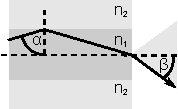
\includegraphics[width=0.35\textwidth]{2016-lahg-04-kiud}
\end{center}
\fi


\ifEngStatement
% Problem name: Optical fiber
An optical fiber consists of a cylindrical glass core with a refractive index $n_1=\SI{1,46}{}$ and a coating with a refractive index $n_2=\SI{1,44}{}$ that surrounds the core as a tube. Using classical optics, find the apex angle of a cone of light leaving a long optical fiber.
\fi


\ifEngHint
In a long optic fiber only such rays will be spreading that go through total internal reflection between the interface of the core and the coating.
\fi


\ifEngSolution
In a long optical fiber only such rays will remain that go through a total internal reflection at the separation surface of the core and the coating. If the light falls on the separation surface with a smaller angle than the critical angle of total internal reflection then both reflection and refraction take place. After several reflections the intensity of such rays will practically decrease to zero because almost all the light has refracted out from the sides of the fiber. The critical angle of total internal reflection $\alpha=\arcsin(n_2/n_1)=\SI{80,5}{\degree}$. The rays corresponding to the critical angle are travel at an angle $\SI{90}{\degree}-\alpha$ with respect to the fiber’s axis. After refracting out from the fiber’s end the angle of these rays with respect to the fiber’s axis is $\beta=\arcsin[n_1\sin(\SI{90}{\degree}-\alpha)]=\arcsin[n_1\cos(\alpha)]$. The light cone’s apex angle $\theta$ is two times bigger than that: $\theta=2\beta=2\arcsin[n_1\cos(\alpha)]=\SI{28}{\degree}$. Because $\cos(\arcsin(a))=\sqrt{1-a^2}$ then the answer can be presented as $\theta=2\arcsin(\sqrt{n_1^2-n_2^2})$.
\begin{center}
    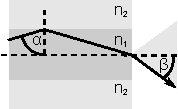
\includegraphics[width=0.35\textwidth]{2016-lahg-04-kiud}
\end{center}
\fi
}